\section{Front-end}


\subsection{Diagramma dei package}


\subsection{Diagramma delle classi}

\begin{figure}[H]
\centering
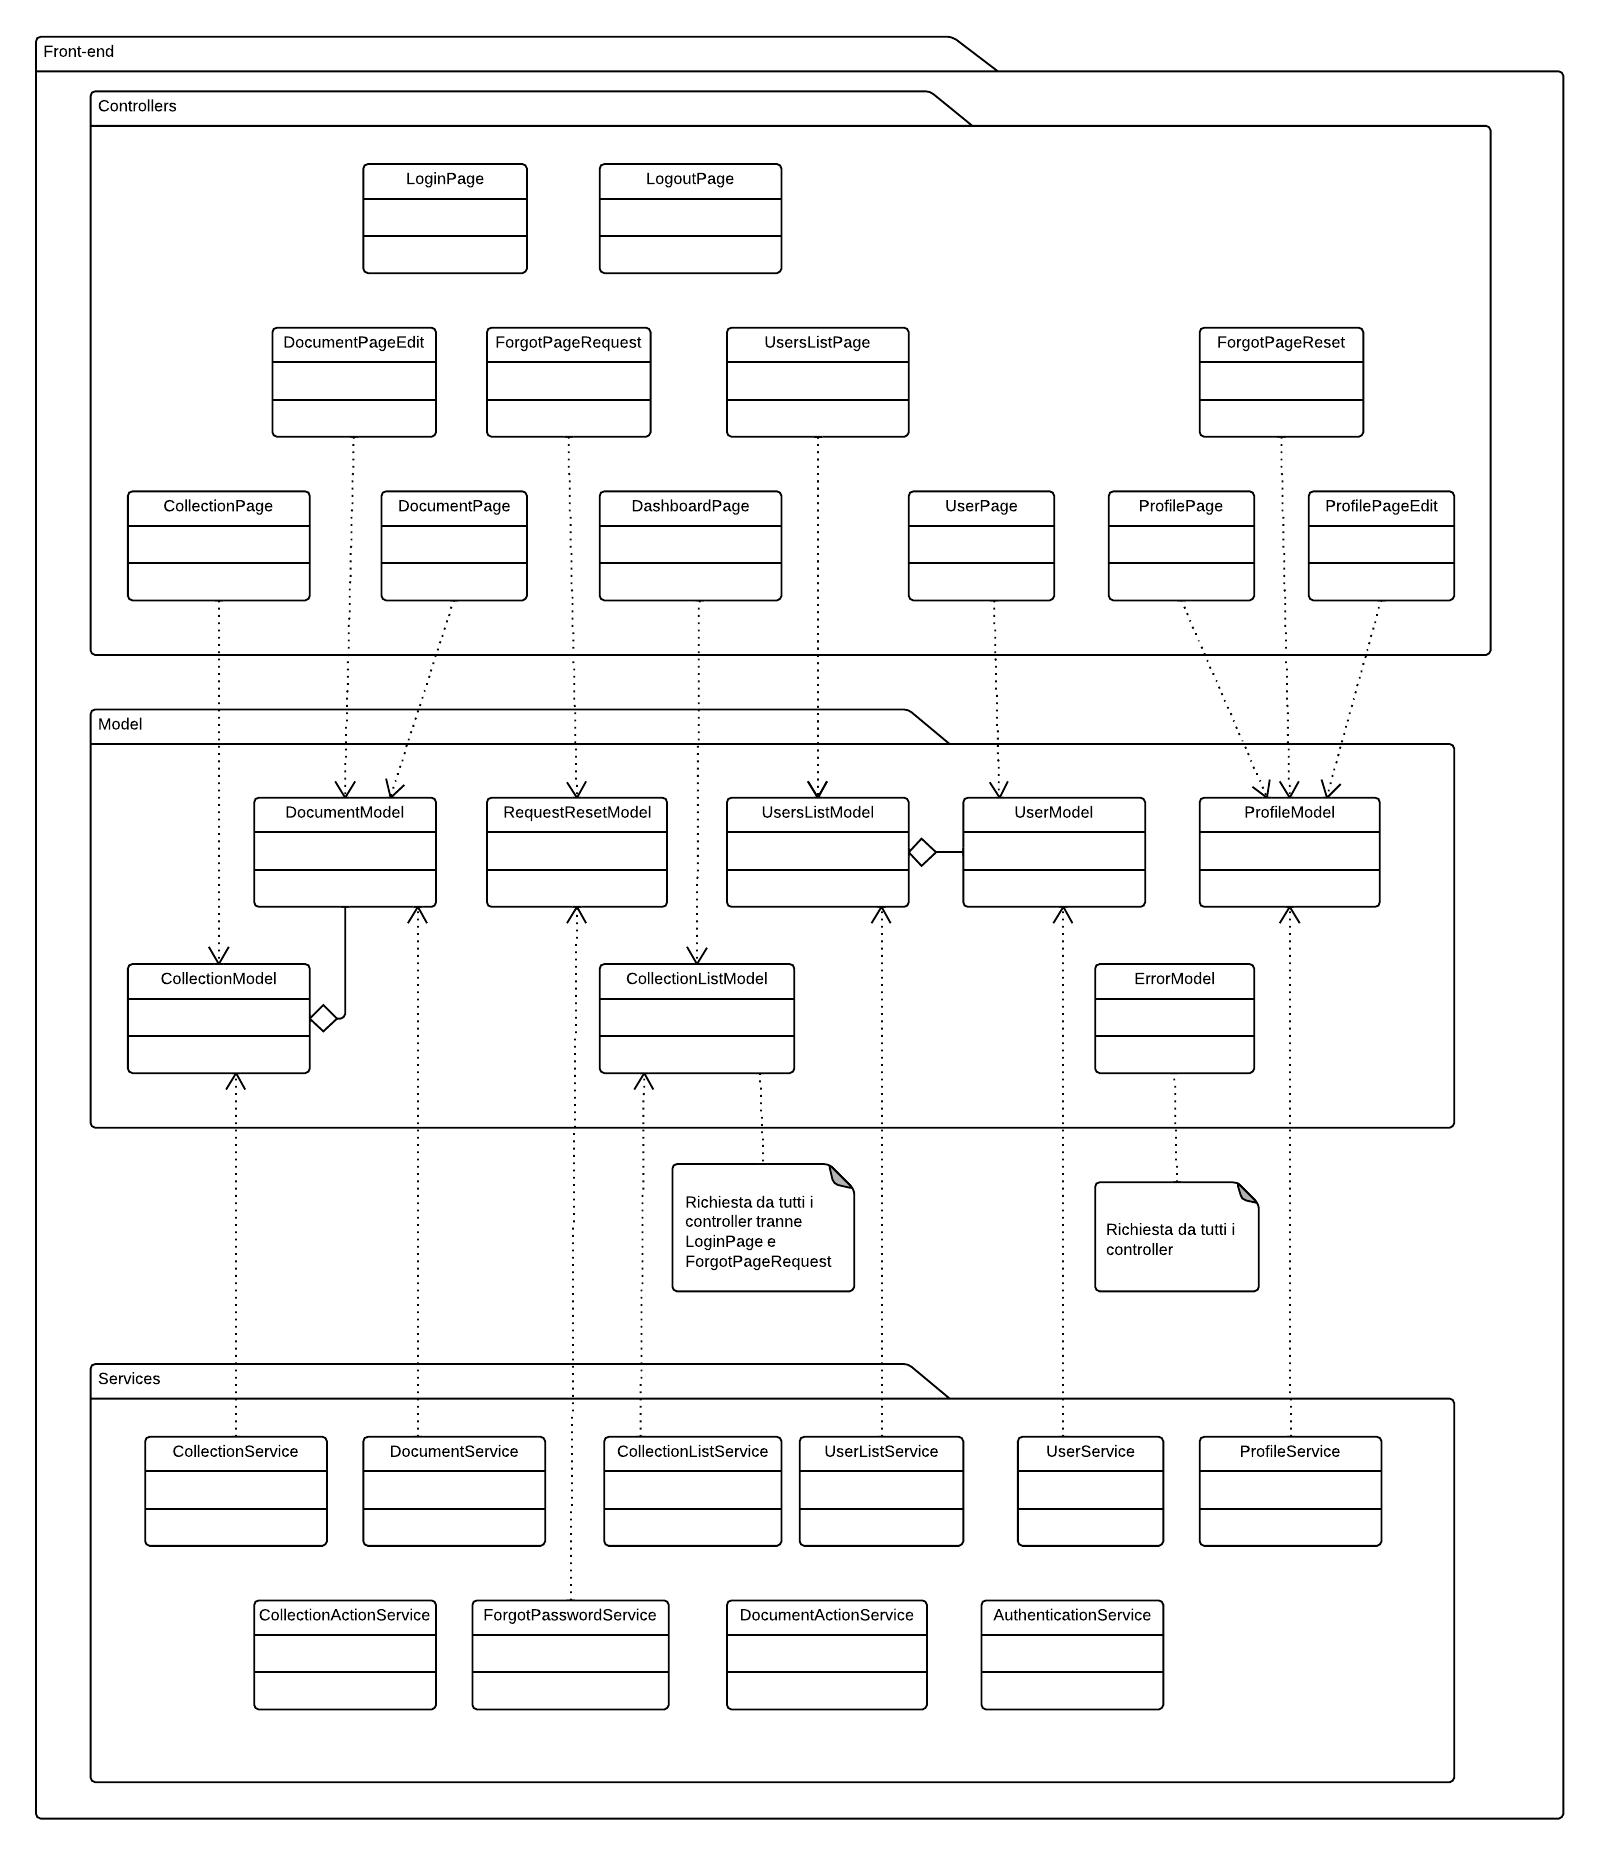
\includegraphics[width=\textwidth]{uml/diagramma-classi-front-end.png}
\caption{Diagramma delle classi del Front-end}
\label{diagrammaClassiFrontEnd}
\end{figure}

TODO: per ogni classe spiegare in poche righe
- Descrizione (per scriverla si risponde alla domanda ``cos'è?'')
- Utilizzo (per scriverla si risponde alla domanda ``a cosa serve?'')

Tutto questo dovrebbe potersi fare da Requisteak...
